\chapter{Implementacija i korisničko sučelje}
		
		
		\section{Korištene tehnologije i alati}
		
			 
			 Tim je za potrebe komunikacije koristio \underline{WhatsApp}\footnote{https://www.whatsapp.com/} aplikaciju i \underline{Discord}\footnote{https://discord.com/} platformu. WhatsApp je služio za osnovnu komunikaciju poput dogovora sastanaka i prenošenje najbitnijih informacija o napretku projekta. Za online sastanke se koristio Discord jer je omogućavao jednostavno spajanje u glasovni poziv i dijeljenje ekrana drugim članovima tima, a uz to nudi i mogućnost organiziranja različitih kanala kako bi komunikacija među podtimovima (\textit{frotend}, \textit{backend}) bila organizirana. Korišteni sustav za upravljanje izvornim kodom je \underline{Git}\footnote{https://git-scm.com/}, a udaljeni repozitorij je postavljen na web platformu \underline{GitLab}\footnote{https://about.gitlab.com/}. \par
			 
			 Za pisanje dokumentacije je bio korišten \underline{Overleaf}\footnote{https://www.overleaf.com/} što je cloud-based LaTeX editor zahvaljujući kojem je dokumentacija s aktualnim promjenama bila dostupna svakom članu bez dodatnih instalacija. Kao provjeru pravopisa koristili smo online alat \underline{ispravi.me}\footnote{https://ispravi.me/}. UML dijagrame izrađivali smo u alatu \underline{Astah UML}\footnote{https://astah.net/products/astah-uml/}, a dijagram baze podataka izrađen je u alatu \underline{dbdiagram.io}\footnote{https://dbdiagram.io/home}. \par
			 
			 Odabrano razvojno okruženje za našu aplikaciju bio je \underline{Visual Studio Code}\footnote{https://code.visualstudio.com/} koji ima integrirani terminal i podršku za Git te uključuje podršku za debugiranje. VS Code je odabran zbog toga što je dostupan za sve operacijske sustave koje smo koristili za rad na projektu - Windows, Linux i macOS. \par
			 
            U pisanju aplikacije korišten je  \underline{Flask}\footnote{https://flask.palletsprojects.com/en/2.2.x/} kao radni okvir za programski jezik \underline{Python}\footnote{https://www.python.org/}. Uz to je korišten i alat \underline{pipenv}\footnote{https://pipenv.pypa.io/en/latest/} koji pomaže pri stvaranju virtualnog okruženja za \textit{backend} dio aplikacije te alat \underline{SQLAlchemy}\footnote{https://www.sqlalchemy.org/} koji olakšava korištenje baze podataka i SQL-a u \textit{backendu}. Za izradu \textit{frotenda} koristio se programski jezik \underline{TypeScript}\footnote{https://www.typescriptlang.org/} koji je zapravo omotač za programski jezik \underline{JavaScript}\footnote{https://www.javascript.com/} te ima dodatne funkcionalnosti u odnosu na JavaScript. Također, koristio se \underline{React}\footnote{https://reactjs.org/} koji je JavaScript library, ali ga se često smatra i radnim okvirom, iako to tehnički nije. \underline{Material UI}\footnote{https://mui.com/}, tj. MUI je jedan od libraryja koji se uvelike koristi u projektu zbog svoje jednostavnosti i povezanosti s Reactom. On nudi i omogućava korištenje već gotovih komponenti te olakšava stvaranje novih. \par
            
            Za prikazivanje mapa u aplikaciji koristio se \underline{Leaflet}\footnote{https://leafletjs.com/}, JavaScript library za interaktivne mape, a za generiranje ruta kartografa koristio se \underline{OSRM}\footnote{https://project-osrm.org/}, open source alat koji generira najkraću rutu za obilazak željenih točaka.
            
            Baza podataka nalazi se na cloud poslužitelju \underline{Render}\footnote{https://render.com/}, a \textit{frotend} i \textit{backend}  postavljeni su na web poslužitelju \underline{DigitalOcean}\footnote{https://www.digitalocean.com/}. \par
			
			
			\eject 
		
	
		\section{Ispitivanje programskog rješenja}
			
			\textbf{\textit{dio 2. revizije}}\\
			
			 \textit{U ovom poglavlju je potrebno opisati provedbu ispitivanja implementiranih funkcionalnosti na razini komponenti i na razini cijelog sustava s prikazom odabranih ispitnih slučajeva. Studenti trebaju ispitati temeljnu funkcionalnost i rubne uvjete.}
	
			
			\subsection{Ispitivanje komponenti}
			\textit{Potrebno je provesti ispitivanje jedinica (engl. unit testing) nad razredima koji implementiraju temeljne funkcionalnosti. Razraditi \textbf{minimalno 6 ispitnih slučajeva} u kojima će se ispitati redovni slučajevi, rubni uvjeti te izazivanje pogreške (engl. exception throwing). Poželjno je stvoriti i ispitni slučaj koji koristi funkcionalnosti koje nisu implementirane. Potrebno je priložiti izvorni kôd svih ispitnih slučajeva te prikaz rezultata izvođenja ispita u razvojnom okruženju (prolaz/pad ispita). }
			
			
			
			\subsection{Ispitivanje sustava}
			
			 \textit{Potrebno je provesti i opisati ispitivanje sustava koristeći radni okvir Selenium\footnote{\url{https://www.seleniumhq.org/}}. Razraditi \textbf{minimalno 4 ispitna slučaja} u kojima će se ispitati redovni slučajevi, rubni uvjeti te poziv funkcionalnosti koja nije implementirana/izaziva pogrešku kako bi se vidjelo na koji način sustav reagira kada nešto nije u potpunosti ostvareno. Ispitni slučaj se treba sastojati od ulaza (npr. korisničko ime i lozinka), očekivanog izlaza ili rezultata, koraka ispitivanja i dobivenog izlaza ili rezultata.\\ }
			 
			 \textit{Izradu ispitnih slučajeva pomoću radnog okvira Selenium moguće je provesti pomoću jednog od sljedeća dva alata:}
			 \begin{itemize}
			 	\item \textit{dodatak za preglednik \textbf{Selenium IDE} - snimanje korisnikovih akcija radi automatskog ponavljanja ispita	}
			 	\item \textit{\textbf{Selenium WebDriver} - podrška za pisanje ispita u jezicima Java, C\#, PHP koristeći posebno programsko sučelje.}
			 \end{itemize}
		 	\textit{Detalji o korištenju alata Selenium bit će prikazani na posebnom predavanju tijekom semestra.}
			
			\eject 
		
		
		\section{Dijagram razmještaja}
			
%	\textbf{\textit{dio 2. revizije}}\\
			
%	\textit{Potrebno je umetnuti \textbf{specifikacijski} dijagram razmještaja i opisati ga. Moguće je umjesto specifikacijskog dijagrama razmještaja umetnuti dijagram razmještaja instanci, pod uvjetom da taj dijagram bolje opisuje neki važniji dio sustava.}\\
			
			Na slici \ref{fig:DeploymentDiagram} prikazan je specifikacijski dijagram razmještaja. Iz njega lako možemo iščitati topologiju našeg sustava te odnos između sklopovskih i programskih komponenti. Kao što vidimo, korisnici (administratori, igrači i kartografi) internetskim preglednikom pristupaju web-aplikaciji. Komunikacija između korisničkog i poslužiteljskog računala odvija se preko HTTP veze. Web browser šalje HTTP serveru \textit{HTTP request} na port 3000. HTTP server ovisan je o web-poslužitelju aplikacije, u našem slučaju DigitalOcean, na kojem se nalazi GlobeRunner. Svi potrebni podaci za ispravan rad aplikacije spremaju se u globe-runner bazu podataka koja je "deployana" na Render poslužitelju. Dohvaćanje tih podataka odvija se tako da aplikacija šalje \textit{Data request} na port 5432. Također, u slučaju registracije novog korisnika (igrača ili kartografa) aplikacija SMTP protokolom šalje email s linkom za potvrdu kreiranja profila. Pretpostavljamo da tada korisnici taj isti mail primaju IMAP protokolom dok se spajaju na poslužitelja e-pošte.

			 \begin{figure}[H]
        			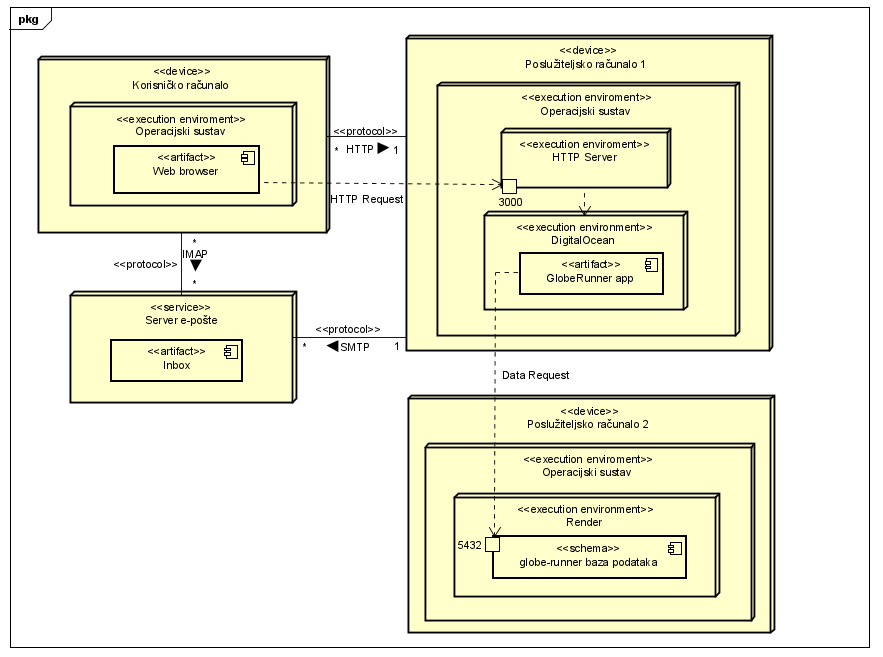
\includegraphics[width=\textwidth]{slike/deploymentdiagram.png}
        			\centering
        			\caption{Dijagram razmještaja}
        			\label{fig:DeploymentDiagram}
        		\end{figure}
			
			\eject 
		
		\section{Upute za puštanje u pogon}
		    Pokretanje aplikacije na vlastitom računalu zahtjeva postavljanje PostgeSQL baze za podatke aplikacije te Redis baze za session-e. Ovdje će postupak za to biti opisan koristeći usluge Render servisa s obzirom da su sve usluge potrebne za ovo besplatne. Cijelo pokretanje projekta radimo preko Docker-a.
		    \\
		
			\textbf{Postavljanje baze podataka na Render servisu}
			
			\begin{enumerate}
			    \item Otvoriti \href{https://render.com/}{render.com} i registrirati se.
			    \item Napraviti novu PostgreSQL bazu. Ime odabrati proizvoljno.
			    
			    \begin{figure}[H]
        			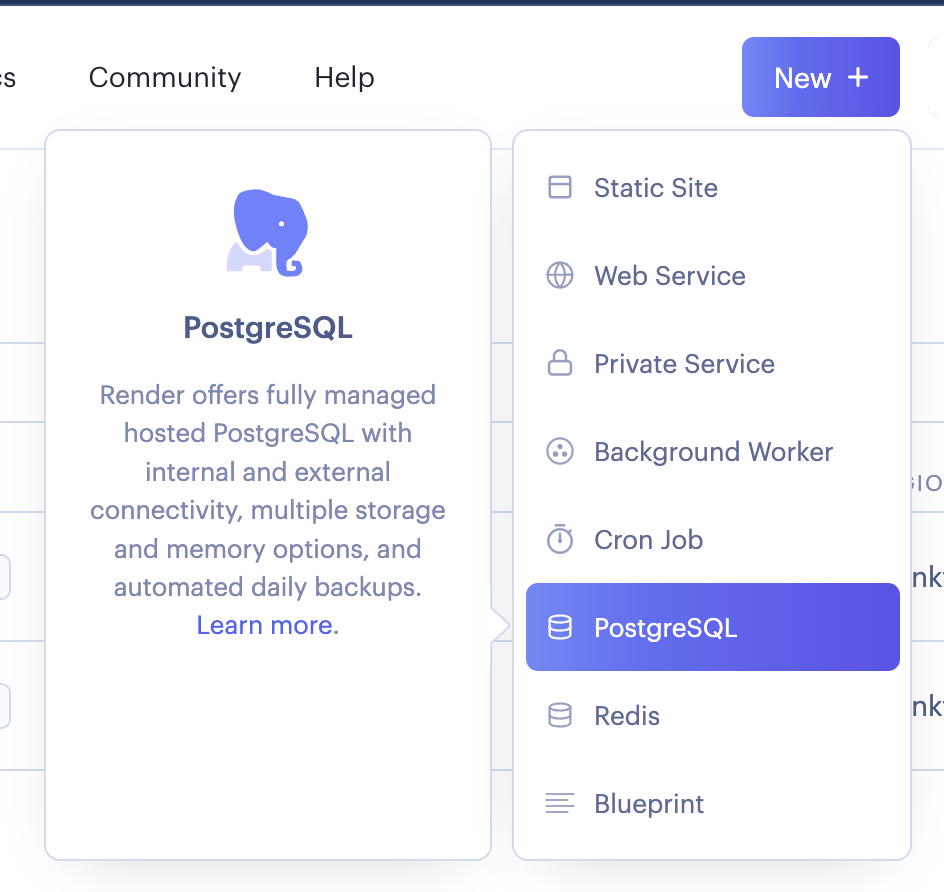
\includegraphics[width=\textwidth]{slike/Upute za puštanje u pogon/create_db.png}
        			\centering
        		\end{figure}
        		
        		\begin{figure}[H]
        			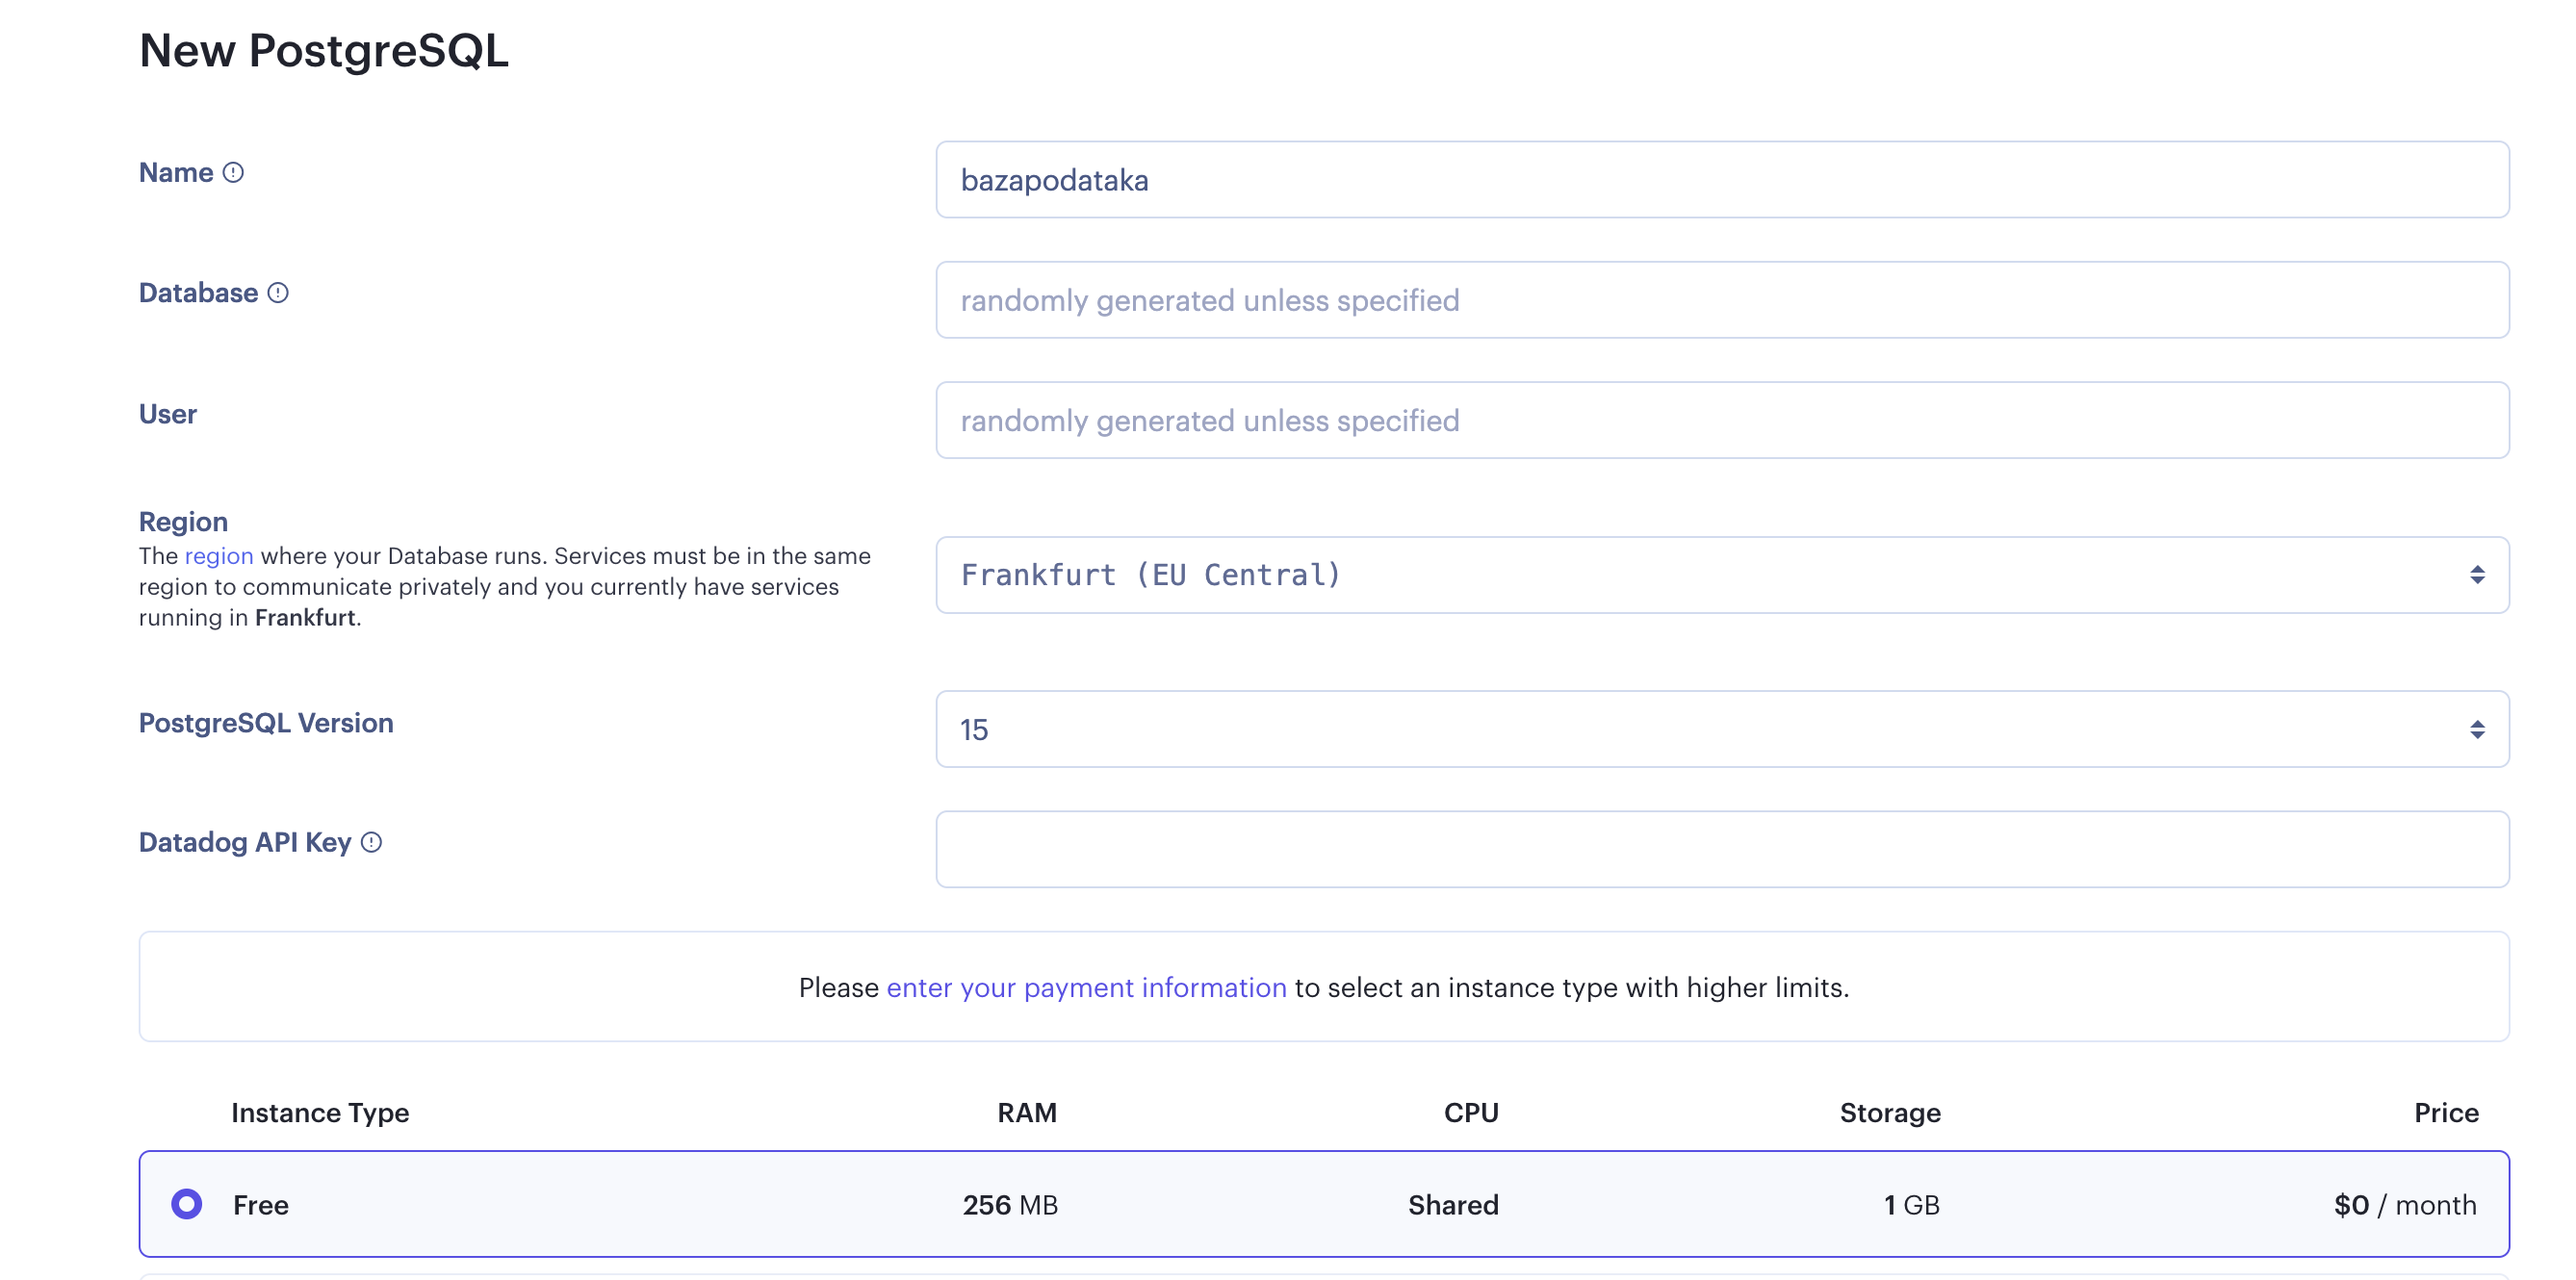
\includegraphics[width=\textwidth]{slike/Upute za puštanje u pogon/db_settings.png}
        			\centering
        		\end{figure}
        		
        		\item Otvoriti Dashboard i kliknuti na upravo kreiranu bazu.
        		\item Podaci na dnu u Info prozoru pod Connections će nam trebati za spajanje aplikacije s bazom.
        		
        		\begin{figure}[H]
        			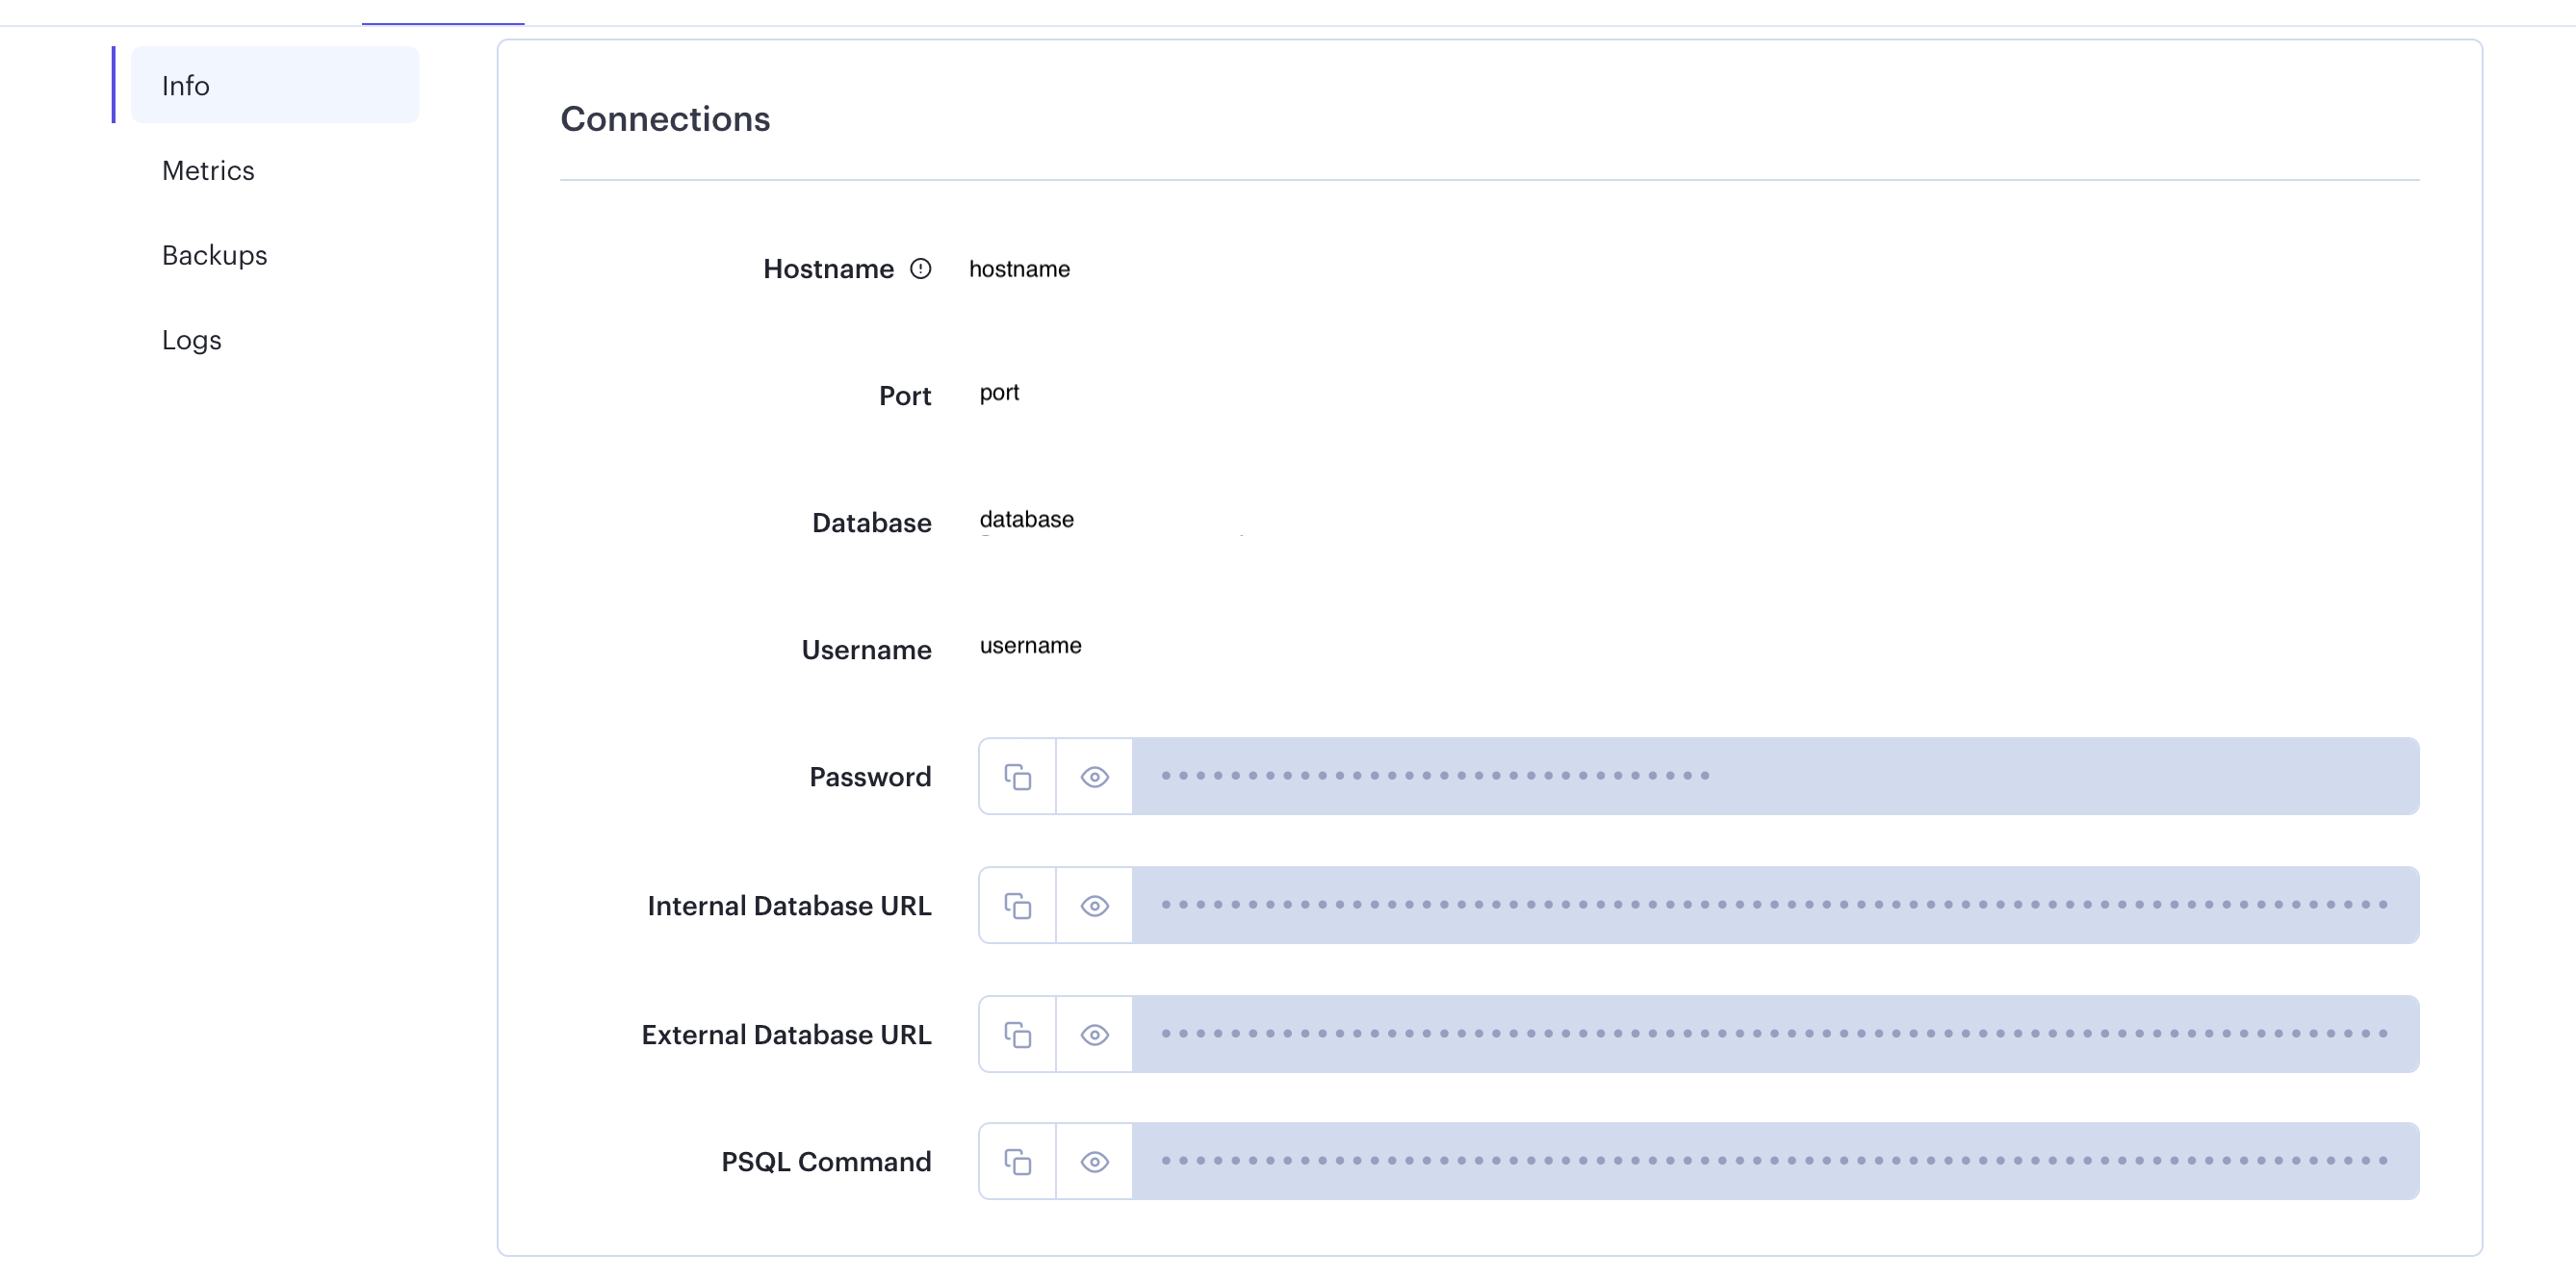
\includegraphics[width=\textwidth]{slike/Upute za puštanje u pogon/db_connections.png}
        			\centering
        		\end{figure}
        		
        		\item Pod Access Control treba dodati vlastitu IP računala na kojem će se vrtiti aplikacija.
        		
        		\begin{figure}[H]
        			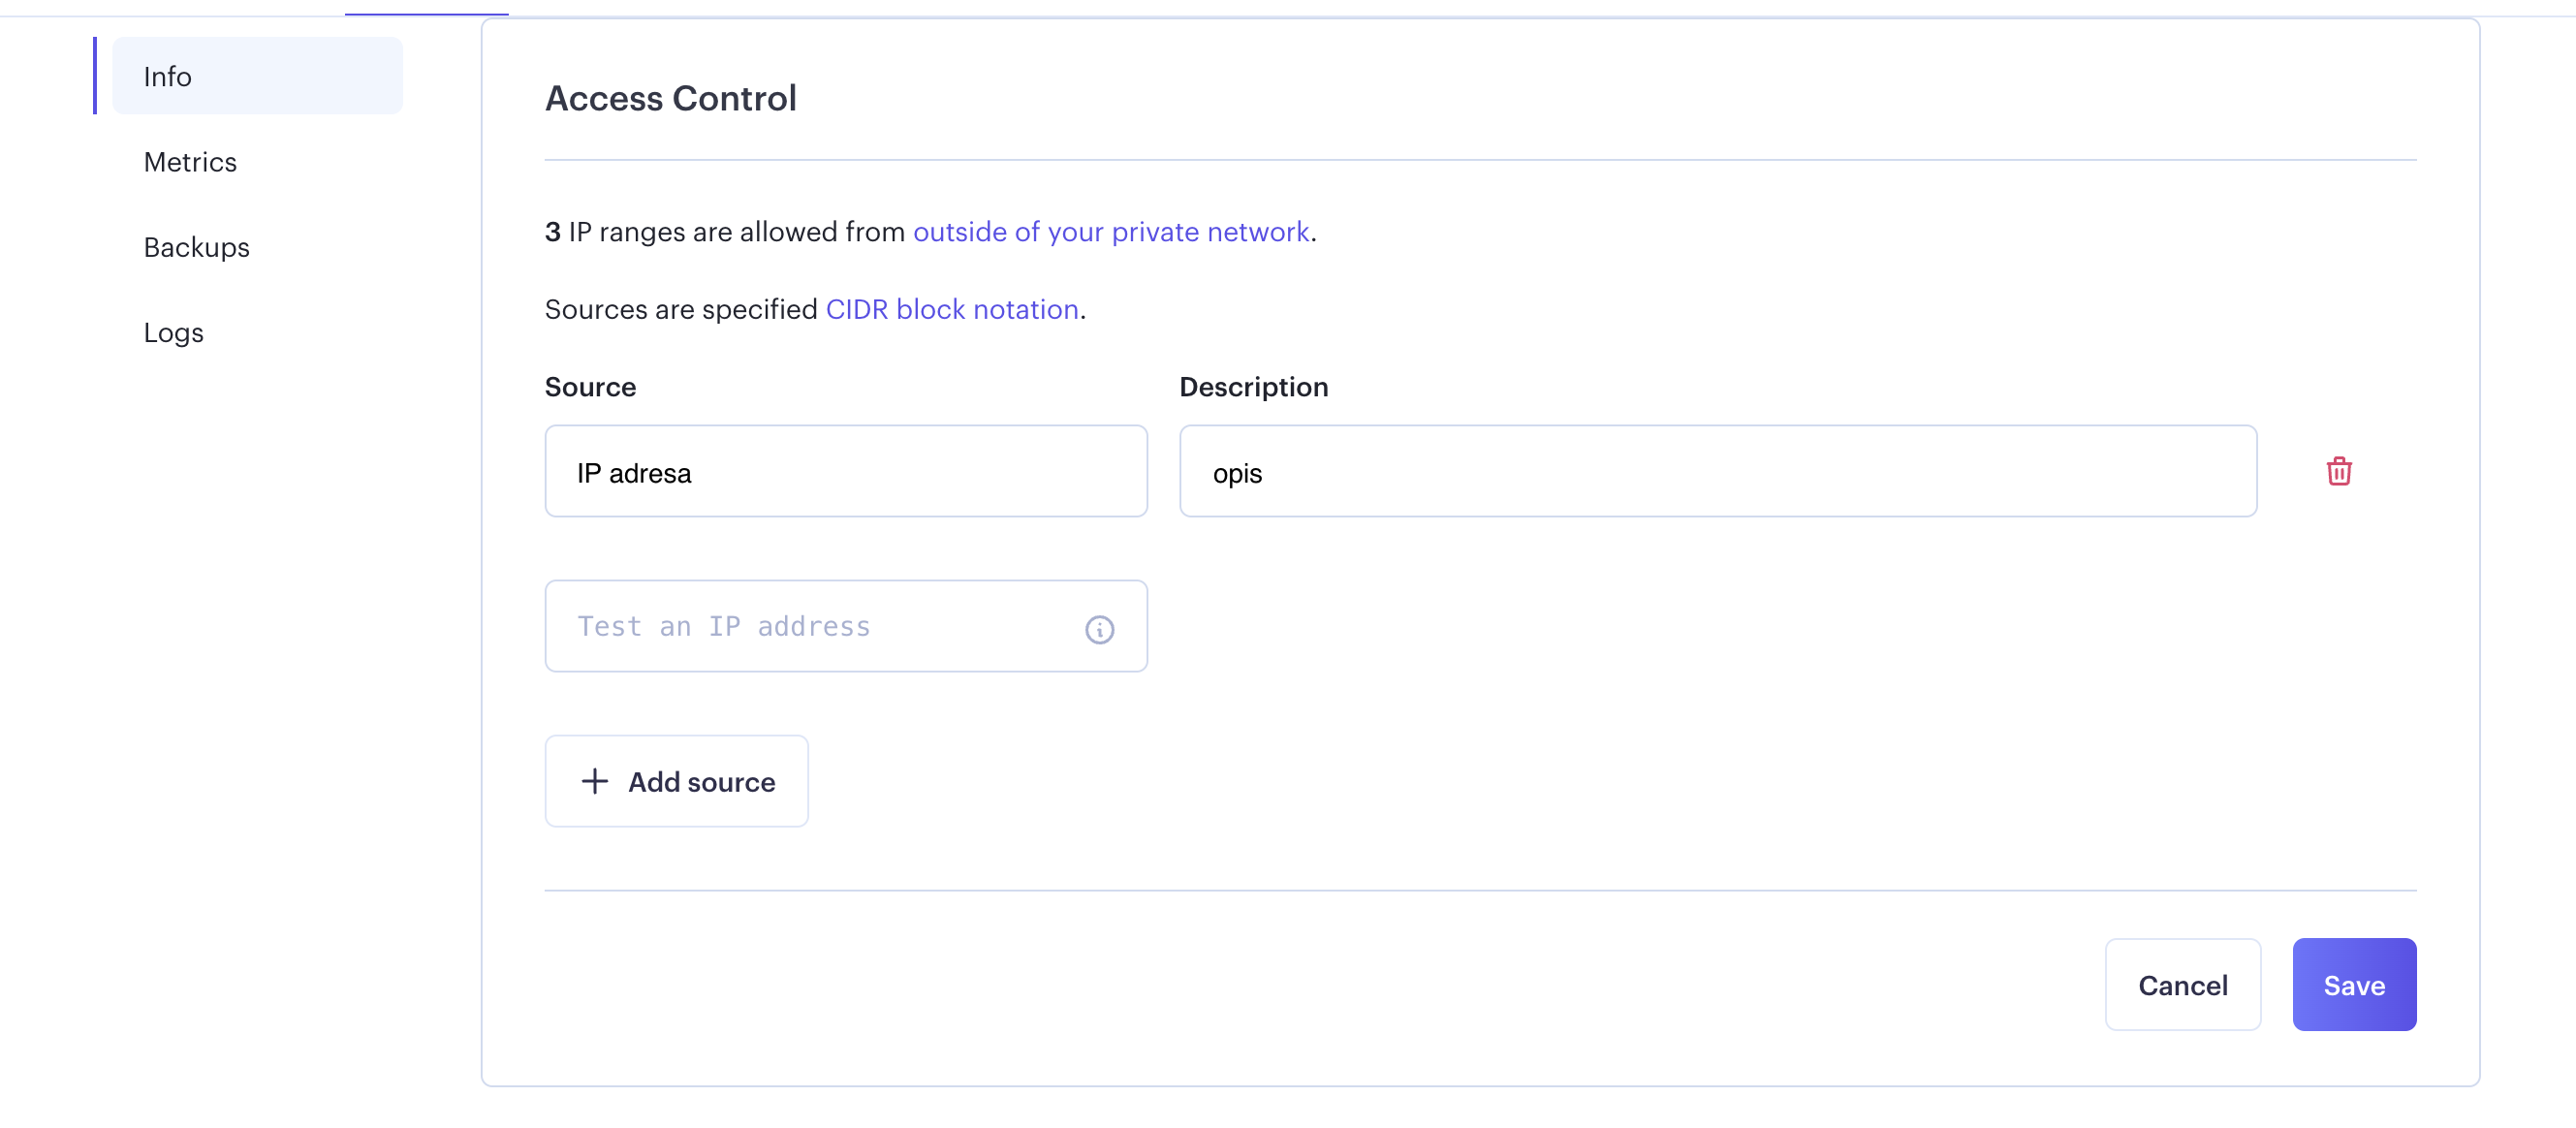
\includegraphics[width=\textwidth]{slike/Upute za puštanje u pogon/db_access.png}
        			\centering
        		\end{figure}
			
			\eject 
			\end{enumerate}
			
			\textbf{Postavljanje Redis baze na Render servisu}
			
			\begin{enumerate}
			    \item Otvoriti \href{https://render.com/}{render.com} i registrirati se.
			    \item Napraviti novu Redis bazu. Ime odabrati proizvoljno.
			    
			    \begin{figure}[H]
        			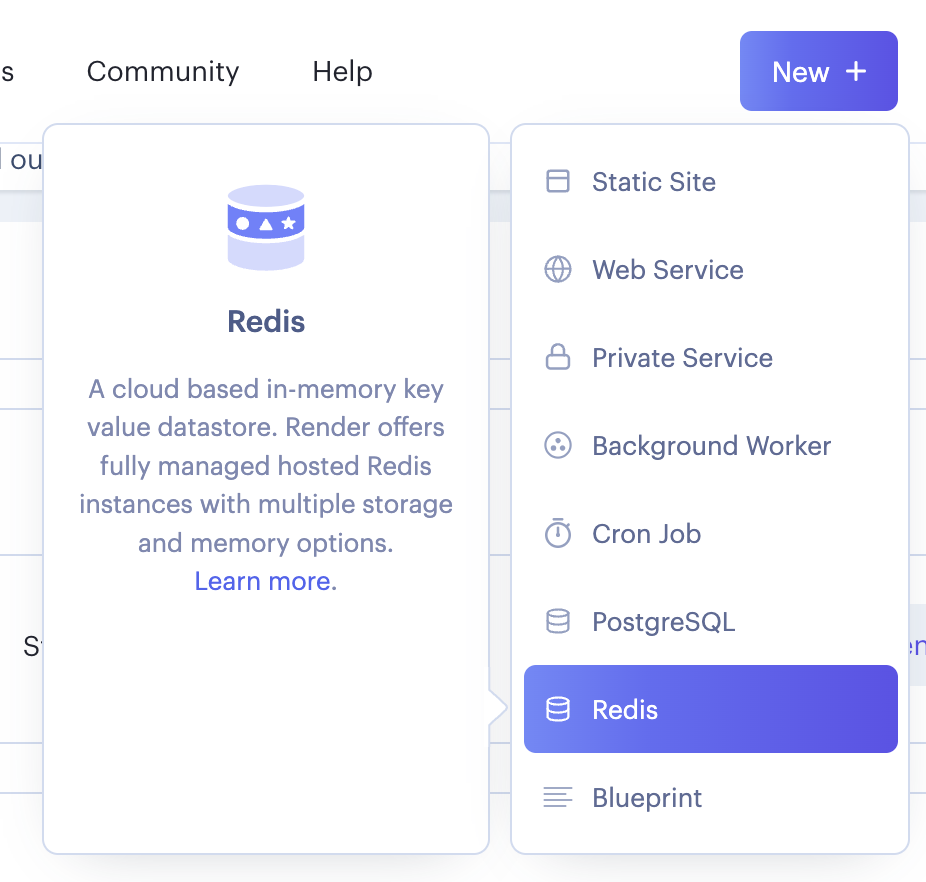
\includegraphics[width=\textwidth]{slike/Upute za puštanje u pogon/redis.png}
        			\centering
        		\end{figure}
        		
        		\begin{figure}[H]
        			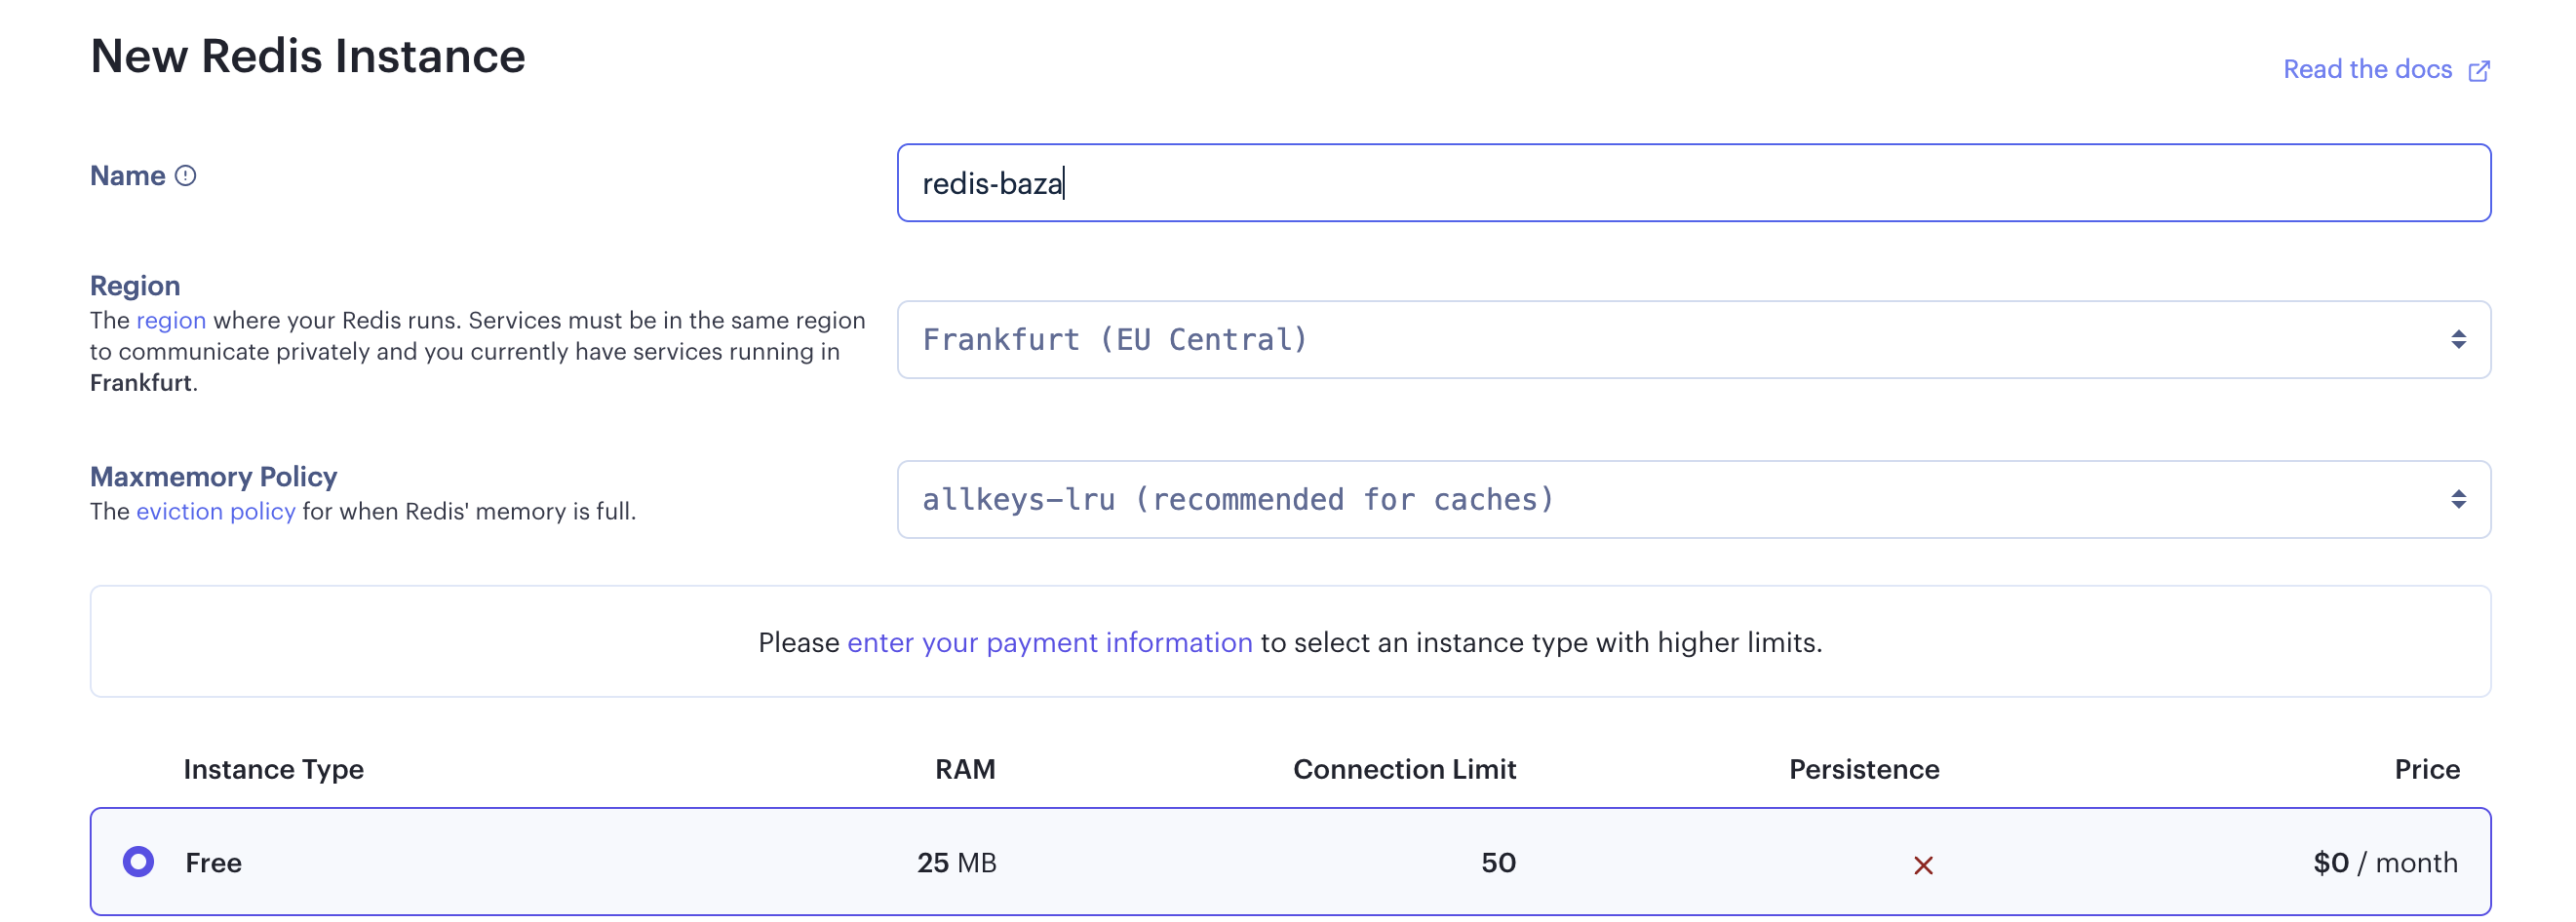
\includegraphics[width=\textwidth]{slike/Upute za puštanje u pogon/new_redis.png}
        			\centering
        		\end{figure}
        		
        		\item Otvoriti Dashboard i kliknuti na upravo kreiranu bazu.
        		
        		\item External Redis URL pod Connections će nam trebati za spajanje aplikacije s bazom.
        		
        		\begin{figure}[H]
        			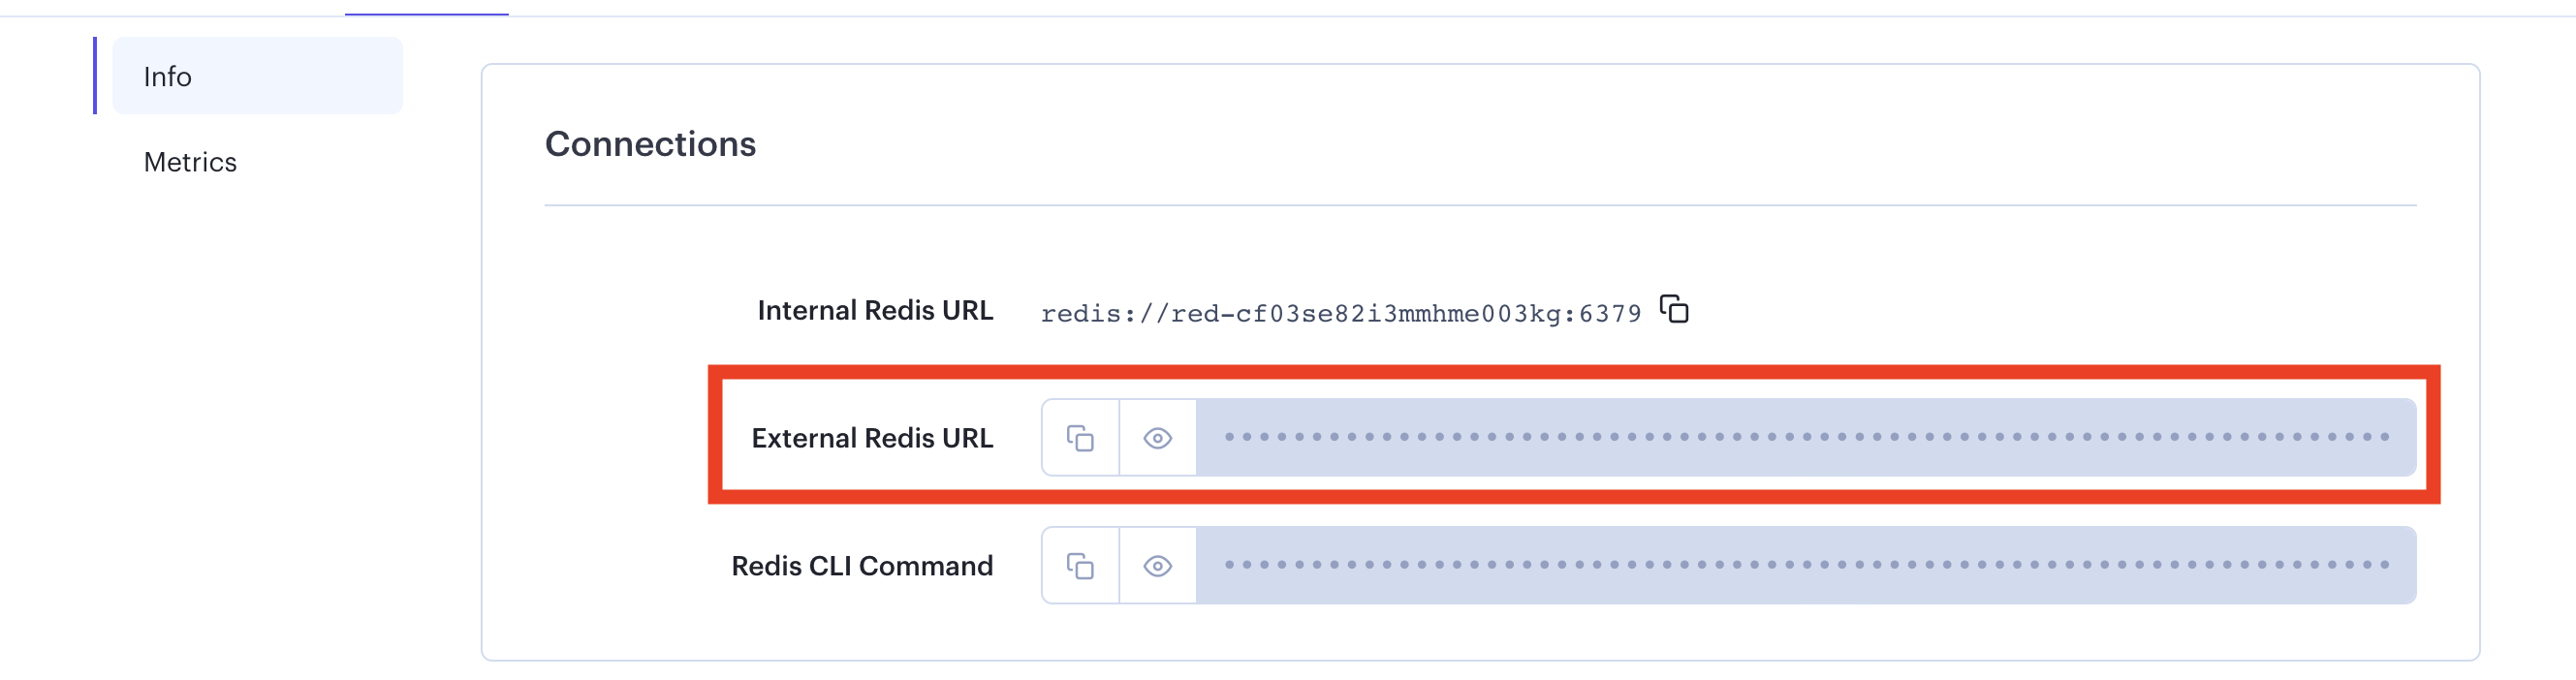
\includegraphics[width=\textwidth]{slike/Upute za puštanje u pogon/external_redis.png}
        			\centering
        		\end{figure}
        		
        		\item Pod Access Control treba dodati vlastitu IP računala na kojem će se vrtiti aplikacija.
        		
        		\begin{figure}[H]
        			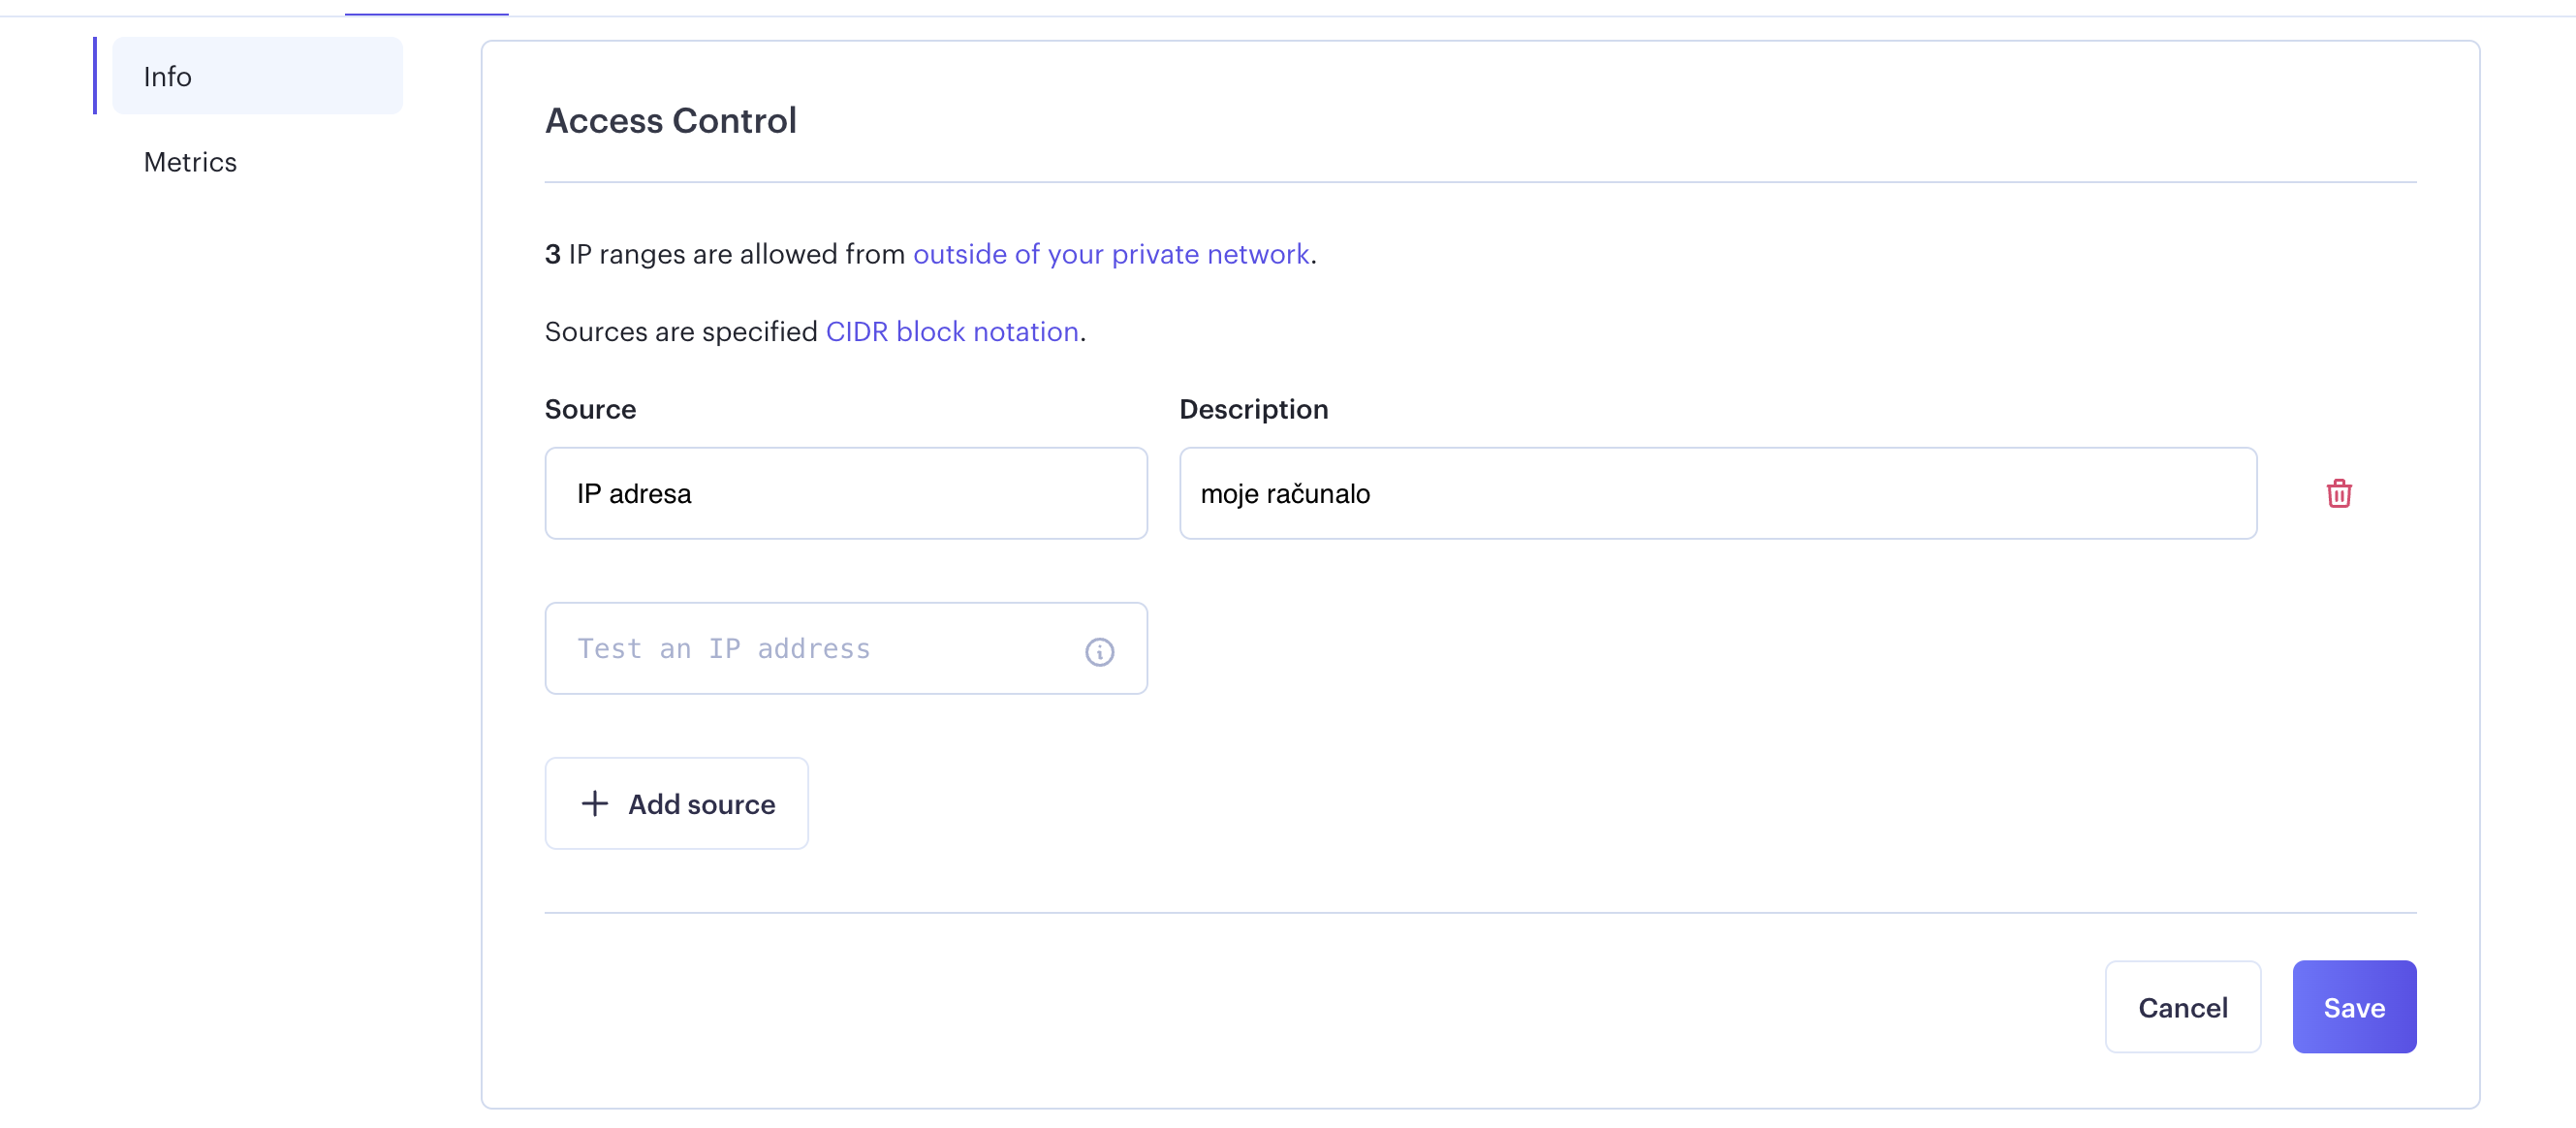
\includegraphics[width=\textwidth]{slike/Upute za puštanje u pogon/redis_access.png}
        			\centering
        		\end{figure}
			    
			\end{enumerate}
			
			\textbf{Pokretanje aplikacije}
			
			\begin{enumerate}
			    \item Instalirati Docker.
			    \item Za slanje mailova treba napraviti gmail account te za njega postaviti lozinku za aplikacije prema sljedećim \href{https://support.google.com/mail/answer/185833?hl=en}{uputama}.
			    \item Klonirati git repozitorij aplikacije na računalo s kojeg će biti pokrenuta aplikacija.
			    \item U IzvorniKod repozitoriju stvoriti .env datoteku čiji sadržaj treba popuniti s podacima o PostgreSQL i Redis bazi te e-mailu.
			\\\textbf{Sadržaj .env datoteke:}
\begin{verbatim}
POSTGRES_PASSWORD = <Password iz Connections podataka za PostgreSQL bazu>
POSTGRES_HOST = <Hostname iz Connections podataka za PostgreSQL bazu>.frankfurt-postgres.render.com
POSTGRES_DB = <Database iz Connections podataka za PostgreSQL bazu>
POSTGRES_USER = <Username iz Connections podataka za PostgreSQL bazu>

REDIS_URL = <External Redis URL>

DEFAULT_FROM_EMAIL = <vlastiti e-mail>
DEFAULT_FROM_EMAIL_PASSWORD = <App password za gore navedeni e-mail>

SECRET_KEY = <proizvoljni niz znakova>
SECURITY_PASSWORD_SALT = <proizvoljni niz znakova>
\end{verbatim}
                \item Iz IzvorniKod repozitorija pokrenuti naredbu \texttt{docker-compose up}.
                \item Otvoriti http://localhost:3000 u browseru.
			 
			\end{enumerate}
			
			\text{}
		
			
			
			\eject 